\section{Mechanical Design}
\label{sec:mechanical}

\subsection{Z-focus-only body}
The imaging head uses a modified OpenFlexure main body with only the Z (focus)
flexure retained; the XY lateral flexure is removed, since lateral motion is
provided by the external rail. The body is printed in PLA
(\texttt{main\_body\_mesoscope.stl}, $\approx\SI{65}{\gram}$) and drives the
optics module along the optical axis via the standard actuator column.

\subsection{Stand and electronics drawer}
A printed stand holds the body and carries a pull-out electronics drawer sized
for the Pi~5, the AI~HAT+ and the RTC (\texttt{microscope\_stand\_mesoscope.stl},
\texttt{electronics\_drawer\_mesoscope.stl}). Board heights and clearances are
documented in \texttt{hardware/stand/openscad/microscope\_stand\_readme.md}.

\subsection{Horizontal tilt and linear rail}
For serial scanning, the whole microscope is tilted \SI{90}{\degree} onto its
side so the optical axis becomes horizontal, resting on the Z-axis motor face.
It is mounted on a carriage on a 2040 V-slot / MGN12 linear rail oriented
perpendicular to the optical path; a bioreactor rack carries the chips in series
on the same structure. A separate rail stepper moves the carriage from chip to
chip (Section~\ref{sec:electronics}). The rail-mount geometry is parametric in
\texttt{hardware/mount/openscad/rail\_mount\_mesoscope.scad}.

\subsection{Bioreactor suspension}
\label{sec:bioreactor}
The chips hang \emph{hochkant} (edge-on) from a fixed suspension so that each is
imaged horizontally through its \SI{16}{\milli\meter} thickness: the
trans-illumination source sits behind the chip row ($+Y$) and the objective in
front ($-Y$). The chips drop into the suspension from above and rest on a
\SI{2}{\milli\meter} rim (\emph{Kranz}); their fluidic tubes exit upward, and the
space \emph{below} the chips stays clear so the tilted imaging head reaches every
station. Suspension and rail share one base plate, fixing the working distance.

Two interchangeable suspension variants exist in the CAD sources. A
metal-spine segmented rack (\texttt{bioreactor\_rack.scad}; renders to
\texttt{bioreactor\_rack\_n\textit{N}.stl}) carries $N$ chips on a stiff
aluminium extrusion. The printable alternative
(\texttt{bioreactor\_bridge\_split.scad}) splits the suspension into three
printed parts: one continuous bridge board plus two separate end towers
(Fig.~\ref{fig:bridge}). At $N=3$ stations the bridge spans only the station row
plus a short end margin ($\approx\SI{280}{\milli\meter}$), keeping it under the
\SI{300}{\milli\meter} print-bed limit so it prints as a single piece with no
splice. Each bridge end bolts onto a tower top ($2\times$~M3); the slim
\SI{20}{\milli\meter} towers sit just outside the end chips and bolt to the base
plate (M5). Both variants are parametric in the station count $N$ and the pitch.
\todo{confirm the chip pitch (\SI{80}{\milli\meter} assumed) and the suspension
geometry against the physical chips, milestone~M3.}

\begin{figure}[!t]
  \centering
  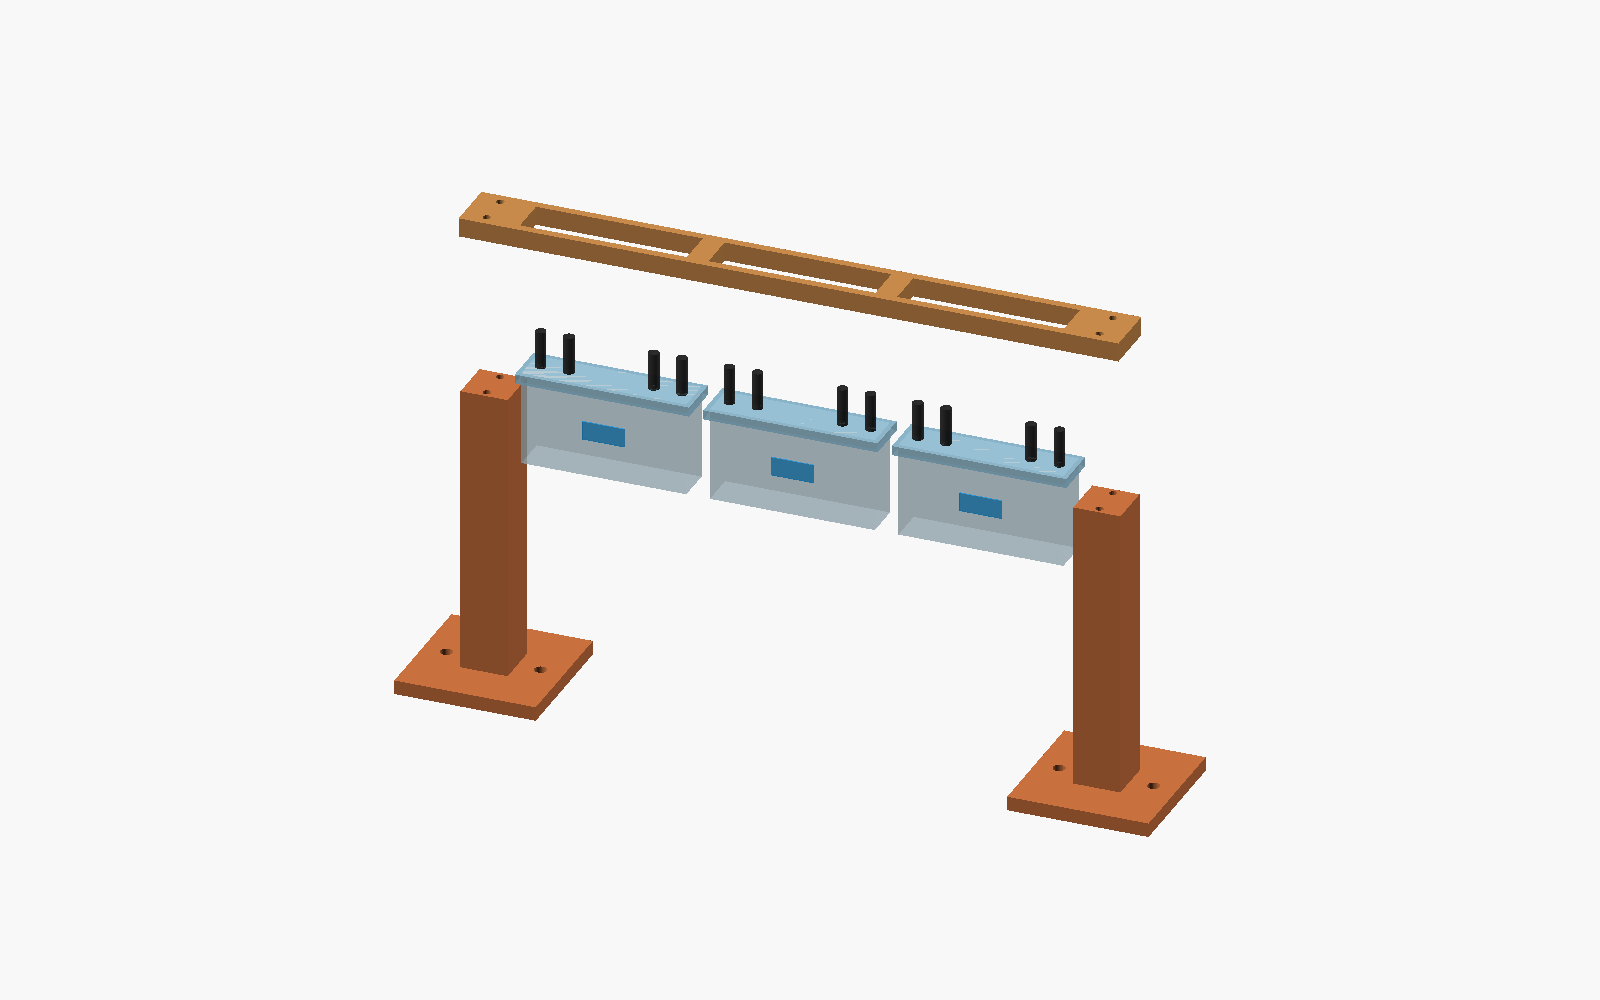
\includegraphics[width=\columnwidth]{bridge_split_exploded.png}
  \caption{Exploded view of the printable bioreactor bridge at $N=3$: one
  one-piece bridge board lifted off its two end towers (three printed parts).
  The chips (semi-transparent reference solids) hang edge-on through the bridge
  and are imaged horizontally. Rendered with OpenSCAD from
  \texttt{hardware/rails/openscad/bioreactor\_bridge\_split.scad}.}
  \label{fig:bridge}
\end{figure}

\subsection{Exploded view}
Fig.~\ref{fig:exploded} shows the exploded upright stack, rendered from the CAD
sources in \texttt{hardware/assembly/} (run \texttt{build\_exploded.sh}; the PNGs
are not committed). Front, opposite-side and unlabelled variants are available.

\begin{figure}[!t]
  \centering
  % rendered by hardware/assembly/build_exploded.sh (not committed to git)
  \figorplaceholder{exploded_view_nolabels.png}{\columnwidth}
  \caption{Exploded view of the upright mesoscope stack: stand and electronics
  drawer, Z-focus body, Z actuator and motor, HQ-camera optics module,
  objective, sample/bioreactor chip and illumination. Rendered with OpenSCAD
  from \texttt{hardware/assembly/openscad/exploded\_view.scad}. Some PCBs, the
  camera, the chip and the LED are simplified placeholder solids.}
  \label{fig:exploded}
\end{figure}

\subsection{Print parameters and tolerances}
Parts print in PLA at \SI{0.2}{\milli\meter} layer height, three perimeters and
\SIrange{20}{30}{\percent} infill. Per-part masses, volumes and print times are
listed in Table~\ref{tab:printed} (Appendix~\ref{sec:appendix}); the print
checklist is in \texttt{hardware/PRINT\_CHECKLIST.md}.
